% Created 2018-02-12 Mon 19:42
\documentclass[sigconf]{acmart}
\usepackage[utf8]{inputenc}
\usepackage[T1]{fontenc}
\usepackage{fixltx2e}
\usepackage{graphicx}
\usepackage{longtable}
\usepackage{float}
\usepackage{wrapfig}
\usepackage{rotating}
\usepackage[normalem]{ulem}
\usepackage{amsmath}
\usepackage{textcomp}
\usepackage{marvosym}
\usepackage{wasysym}
\usepackage{amssymb}
\usepackage{hyperref}
\tolerance=1000
\usepackage{minted}
\usepackage{cuted}
\usepackage[T1]{fontenc}
\usepackage{lmodern}
\usepackage{graphicx}
\usepackage{amsmath}
\usepackage[margin=0.5in]{geometry}
\author{Akash Ganesan}
\affiliation{%
}
\email{akaberto@umich.edu}
\author{Divyansh Pal}
\affiliation{%
}
\email{divpal@umich.edu}
\author{Karthik Muthuraman}
\affiliation{%
}
\email{mkarthik@umich.edu}
\author{Shubham Dash}
\affiliation{%
}
\email{shudbhamd@umich.edu}
\settopmatter{printacmref=false} % Removes citation information below abstract
\renewcommand\footnotetextcopyrightpermission[1]{} % removes footnote with conference information in first column
\pagestyle{plain} % removes running headers
\begin{CCSXML}
<ccs2012>
<concept>
<concept_id>10010147.10010178.10010179.10010182</concept_id>
<concept_desc>Computing methodologies~Natural language generation</concept_desc>
<concept_significance>500</concept_significance>
</concept>
<concept>
<concept_id>10010147.10010178.10010224.10010225.10010227</concept_id>
<concept_desc>Computing methodologies~Scene understanding</concept_desc>
<concept_significance>500</concept_significance>
</concept>
<concept>
<concept_id>10010147.10010178.10010224.10010245.10010250</concept_id>
<concept_desc>Computing methodologies~Object detection</concept_desc>
<concept_significance>500</concept_significance>
</concept>
</ccs2012>
<ccs2012>
<concept>
<concept_id>10010147.10010178.10010224.10010225.10010231</concept_id>
<concept_desc>Computing methodologies~Visual content-based indexing and retrieval</concept_desc>
<concept_significance>500</concept_significance>
</concept>
</ccs2012>
\end{CCSXML}
\ccsdesc[500]{Computing methodologies~Object detection}
\ccsdesc[500]{Computing methodologies~Natural language generation}
\ccsdesc[500]{Computing methodologies~Scene understanding}
\ccsdesc[500]{Computing methodologies~Visual content-based indexing and retrieval}
\date{\today}
\title{Video Based Contextual Question Answering}
\hypersetup{
  pdfkeywords={},
  pdfsubject={},
  pdfcreator={Emacs 25.2.2 (Org mode 8.2.10)}}
\begin{document}

\maketitle


\section{Problem Definition}
\label{sec-1}

The problem we are primarily looking to solve aims at building a
contextual Question-Answering model for a given video. The current
methodologies currently provides a robust model to handle
Question-Answering in images, but we are trying to generalize this
approach to be applied on videos. Adding on it the question-answering
model, what we are trying to build should also be able to handle
contextual queries or questions, for example if a frame has an image
of a man and a cat sitting, the model should be able to handle queries
like “where was the cat sitting with respect to the man” or “what is
the man holding in his right hand”, questions which deal with the
context of that particular frame in consideration.  

The questions being asked will focus primarily on binary yes/no
question answering as well as the questions which ask the “What”,
“Why”, “How”, “When” and “Where”.



\section{Challenges}
\label{sec-2}

There are multiple challenges which we have to deal with in order to
successfully build a model which can efficiently handle queries and
answer those with respect to the video in consideration and also
preserve the context embedded in the video.  First challenge would
be to build a contextual linking in between the scene
graphs. Consider an example where a man is eating food in one frame
which is considered as a key frame and in the second frame he is
driving a car, so the link from one scene graph describing one frame
and the second scene graph describing the other frame should be
linked in such a way so that the graph when traversed for finding
out the answers should be representative of how to video is evolving
through time.  Secondly, for gauging the efficiency of our proposed
model we need to fix upon an evaluation metric which can provide a
measure for calculating the efficiency of our model.  One more
interesting challenge which needs to be tackled for building a model
which handles contextual question-answering on videos in general, we
need to look at how scalable the model would be, for example how
efficient would answer retrieval be if the video is a very long.

\section{Prior Work}
\label{sec-3}

Previous related work can be found in the related fields of video
summarization \cite{DBLP:journals/corr/ZhangCSG16a}, image captioning
\cite{k2,d1} and scene graph generation \cite{k1,s2}. We reviewed papers
that propose methods to generate key-frames of interest from a long
video. A major part of our project will draw from works relating to
dense captioning of images and generating scene graphs. There is a
wide body of recent literature which propose novel and optimized
techniques for the aforementioned tasks. Most of these rely on Deep
Learning methods for object detection and captioning and ML and
optimization techniques to generate the scene graphs. Finally, in
terms of evaluation processes, possible test datasets and possible
metrics, there is a wide range of papers and open datasets that can
be relevant to our project \cite{DBLP:conf/cvpr/NohSH16}.



\section{Proposed Methodology}
\label{sec-4}

In our methodology, we first use the video data and find key frames.
For each keyframe, we do semantic segmentation to get different
localized objects, which will serve as our nodes during graph
generation. YOLO and Faster R-CNN are usually used for semantic
segmentation for their speed and accuracy. For our scope we are
considering a dataset that gives us semantic segmentation results on
the frames of the video.  We then use a dense captioning algorithm
to generate captions for each frame based on the dense captioning
algorithm \cite{k2}.  Now, we can use generated captions to form a
scene graph. These scene graphs from captions are generated using
the algorithm mentioned in \cite{s2}. The next step is to link the
scene graphs. This novel step will establish a relation between the
existing scene graph and the incoming scene graph from the current
frame. This will tell what has changed from one frame to the next
and this relationship is important.  We plan to do this by
augmenting our generated scene graph with the difference of the new
and the current scene graph.  

We may ask questions on the image like, “When did the person get in
the car”?, from two adjacent frames that has a person outside the
car and one has the person inside it.  So, the relationship between
the frame needs to be captured.  Individual questions like where is
an object in a frame may be answered by scene analysis from
questions.  However, it is a challenge to ask for relationship
between the frames that we plan to address.


\clearpage
\begin{strip}
\centering
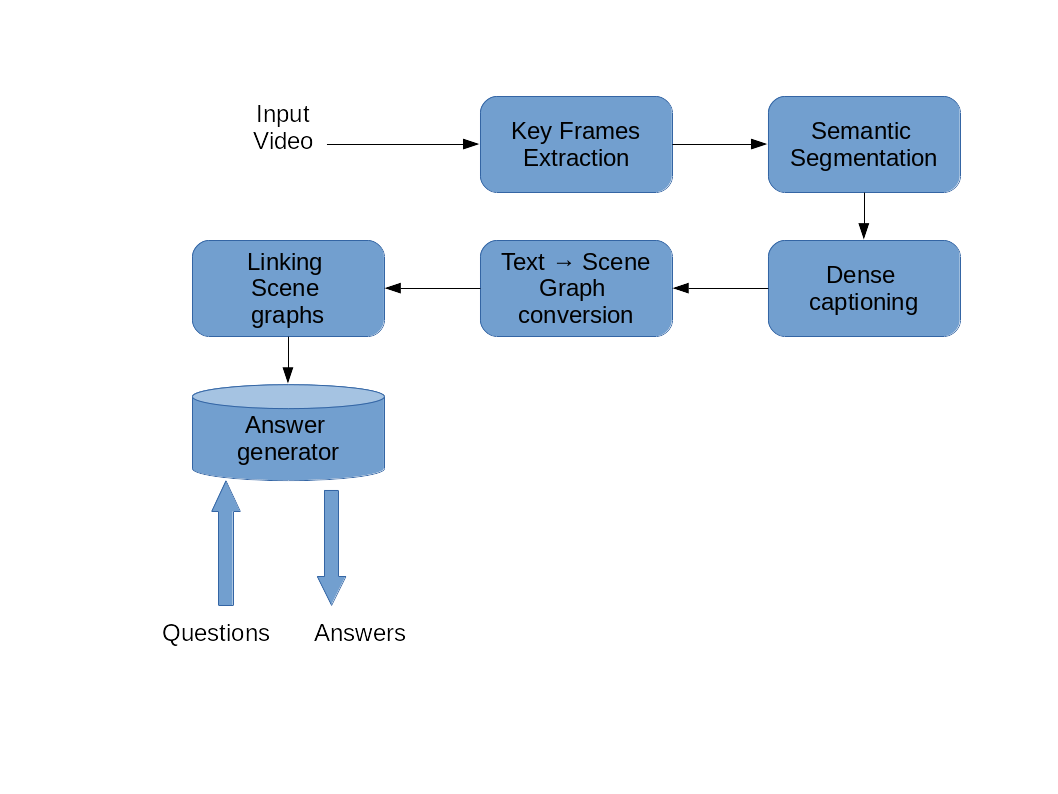
\includegraphics[width=0.8\textwidth]{images/proposal-pipeline.png}
\captionof{figure}{Model pipeline}
\end{strip}  

\section{Dataset Details}
\label{sec-5}
The datasets which are considered for running our experiments are
the Visual Genome and the Youtube-8M databases.  The visual genome
dataset has 108,077 images which has 75,729 unique objects, 40,480
unique objects and the number of unique relationships between those
object, which form the nodes for the respective scene graphs as
40,513.

The second dataset which we will consider for testing our contextual
question-answering model on videos is the Youtube-8M dataset. The
dataset contains frame-by-frame annotations for eight million videos
present.

\section{Evaluation Criteria}
\label{sec-6}
To evaluate the results, we will use Amazon’s mechanical Turk to
generate answers to questions, answered by humans. This provides a
baseline to check the accuracy of the generated answers from our
question-answering model. There are several methods existing for
evaluating the performance of image based question-answering models
such as WUPS, which have been applied to video-based query answering
models.

\section{Future Work}
\label{sec-7}

Our work can be extended to incorporate speech content of video to
generate more node edge combinations. This multimodal approach will
make a denser graph but will store much more contextually rich
information and can be used to answer much more in-depth questions.
Once the graph is generated, a description text of the video can be
generated.  Other attributes of the object can be detected and
incorporated to answer questions about emotion, expression, logic
etc. Currently we focus mainly on actions and relationships but our
work can be extended to emotion and inference based questions.
Lastly, current video retrieval techniques rely heavily on video
metadata such as video title/tags/description etc and less on the
actual content/frames of the video. Extending our work, a video
retrieval system can search on our representation of videos and
hence the actual video content.



\bibliographystyle{ACM-Reference-Format}
\bibliography{manuscript}
% Emacs 25.2.2 (Org mode 8.2.10)
\end{document}